Funktionsweise der Bildverarbeitung


Die Auswertung erfolgt durch visuelle und digitale Analyse.

Die visuelle Beurteilung erfolgt durch die einfache Betrachtung der Verfärbung auf dem Tape. 
Für eine präzisere Analyse errechnet die digitale Bildverarbeitung den Anteil der roten zur weißen Fläche und quantifiziert damit den Flüssigwassergehalt.

Nachdem der Bildausschnitt gewählt wurde, wird das Bild in Grauwerte umgewandelt. mit der RGB Information kann Fehlerkorrektur gemacht werden.

dann wird jeder blob durch einen Kreis mit der gleichen fläche und dem gleichen schwerpunkt ersetzt. auf diesen kreisen kann dann Statistik gemacht werden. die hoffnung ist dass so unterschiedliche geometrien des schnees abgebildet werden können. in \ref{} ist der Code der die übersetzung von schwarzweiß bildern zu die kreise in eine Datenbank speichern übernimmt.
Die Auswahl des Bildausschnitts und Übersetzung in schwarz weiss ist semantisch in 3 dargestellt.



die auswahl des bildausschnitts und übersetzung in schwarz weiss ist sematisch in \ref{fig:Bildverarbeitnugskonzpet} dargestellt.


\begin{figure}
    \centering
    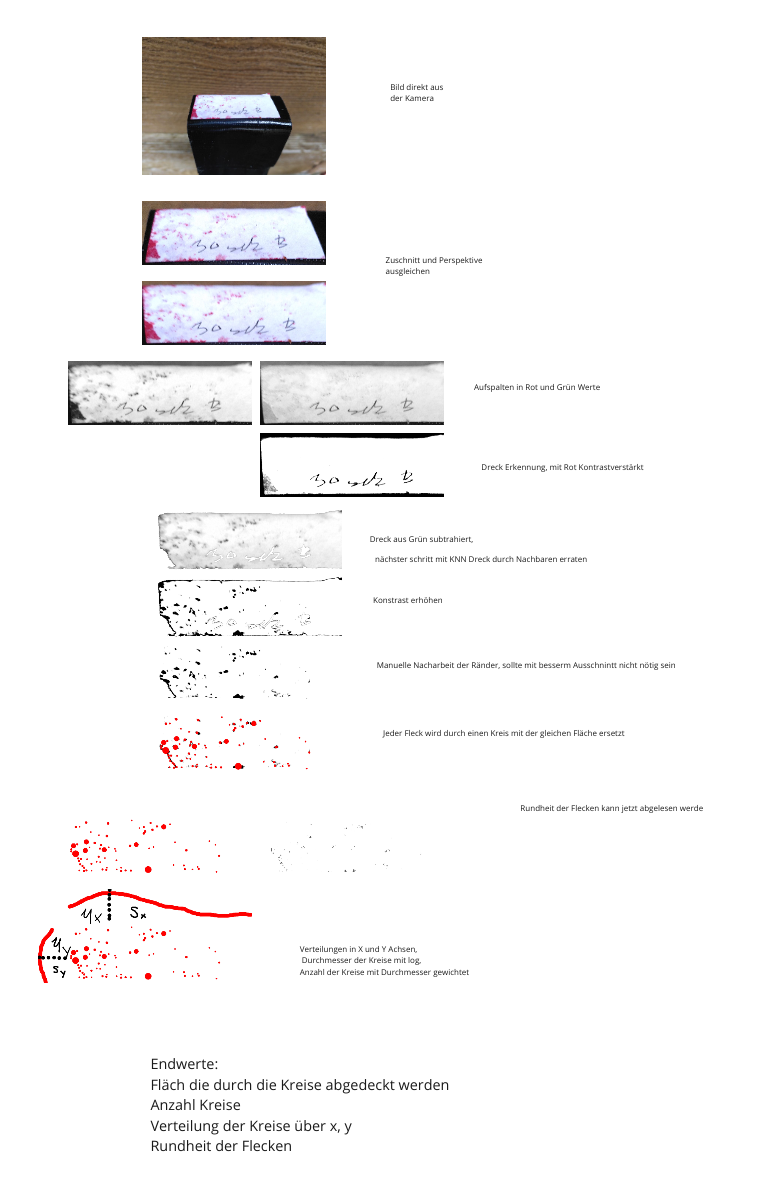
\includegraphics[width=0.8\textwidth]{Bilder/Screenshotfrom2024-04-0112-59-42.png}
    \caption{Bildverarbeitung Konzept}
    \label{fig:Bildverarbeitnugskonzpet}
\end{figure}

\newpage
